\chapter{Pianificazione del progetto} 
\label{cha:pianificazione_del_progetto}	

\section{Introduzione}
In questo documento verrà descritto il processo di sviluppo utilizzato e verrà effettuata la pianificazione delle iterazioni e delle attività da svolgere.

\section{Processo di sviluppo}
\label{sec:processo_di_sviluppo}
Il progetto sarà realizzato secondo la metodologia di sviluppo \gls{rup}.
Tale metodologia prevede quattro fasi sequenziali che possono essere iterate:
\begin{enumerate}
	\item \fase{Inizio}: In cui viene stabilito il caso di business per il sistema.
	\item \fase{Elaborazione}: In cui viene sviluppato e compreso il dominio del problema e l'architettura del sistema.
	\item \fase{Costruzione}: In cui viene effettuta la progettazione, la programmazione e il test del sistema.
	\item \fase{Transizione}: In cui viene stabilito il sistema nell'ambiente di esecuzione.
\end{enumerate}

\noindent
In ognuna di queste fasi possono essere svolte le seguenti attività:
\begin{itemize}
	\item \workflow{Raccolta dei requisiti}
	\item \workflow{Analisi}
	\item \workflow{Progettazione}
	\item \workflow{Implementazione}
	\item \workflow{Test}
\end{itemize}

\noindent
A seconda della fase in cui ci si trova verranno svolte più o meno attività. 
Un tipico esempio di distribuzione delle attività nelle varie fasi è il seguente:
\begin{center}
   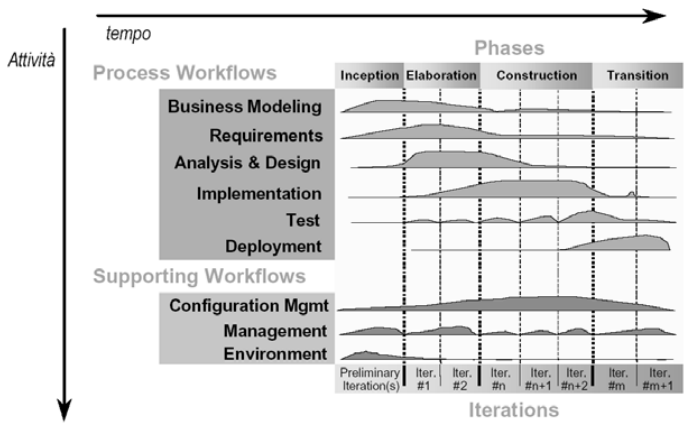
\includegraphics[width=\textwidth]{assets/fasiworkflow}
\end{center}

\section{Pianificazione iterazioni}
\label{sec:pianificazione_iterazioni}
Saranno di seguito elencate le iterazioni svolte durante il progetto, durante lo sviluppo compariranno le iterazioni già effettuate e la pianificazione dell'iterazione successiva.

\tabiter{Iterazione 01}{Inizio}{\begin{itemWork}
							        \item Stesura del documento di richiesta
							        \item Stesura del documento di visione
							        \item Inizio stesura del glossario e degli acronimi
							    \end{itemWork}}{\emptycell}{Effettuata} 

\tabitervspace

\tabiter{Iterazione 02}{Inizio}{% 
    \begin{itemWork}
        \item Studio di fattibilità
        \item Contratto
        \item Aggiornamento glossario e degli acronimi
    \end{itemWork}}{\begin{itemWork}
			    		\item Confermata fattibilità
						\item Stakeholder d’accordo con obiettivi e funzionalità chiave sistema
			   		\end{itemWork}}{Effettuata} 

\tabitervspace

\tabiter{Iterazione 03}{Elaborazione}{
    \begin{itemWork}
    		\item Pianificazione del progetto
	        \item Specifica del sistema
	        \item Aggiornamento del glossario e degli acronimi
    \end{itemWork}}{\emptycell}{In corso}

\tabitervspace

\tabiter{Iterazione 04}{Elaborazione}{
    \begin{itemWork}
	        \item Specifica dei requisiti
	        \item Specifica dei casi d'uso
	        \item Aggiornamento del glossario e degli acronimi
    \end{itemWork}}{\emptycell}{Non effettuata}

\tabitervspace

\tabiter{Iterazione 05}{Elaborazione}{
    \begin{itemWork}
	        \item Aalisi dei rischi
	        \item Analisi dei costi
	        \item Aggiornamento del glossario e degli acronimi
    \end{itemWork}}{\emptycell}{Non effettuata}

\tabitervspace

\tabiter{Iterazione 06}{Elaborazione}{
    \begin{itemWork}
    		\item Creazione schede CRC
	        \item Definizione classi di analisi
	        \item Realizzazione casi d'uso
	        \item Aggiornamento del glossario e degli acronimi
    \end{itemWork}}{\begin{itemWork}
				        \item Creato piano di progetto che permetta di formulare un’offerta realistica				      
				        \item Stakeholder d’accordo su continuare
				    \end{itemWork}}{Non effettuata}

\tabitervspace

\tabiter{Iterazione 07}{Costruzione}{
	\begin{itemWork}
			\item Specifica architettura
	        \item Definizione classi progetto, sottoinsiemi, componenti
	        \item Aggiornamento del glossario e degli acronimi
	\end{itemWork}}{\emptycell}{Non effettuata}

\tabitervspace

\tabiter{Iterazione 08}{Costruzione}{
	\begin{itemWork}
	        \item Cicli di vita di classi significative
			\item Piano dei test
	        \item Completamento del glossario e degli acronimi
	\end{itemWork}}{\begin{itemWork}
					        \item Sistema pronto per beta testing      
				    \end{itemWork}}{Non effettuata}


\begin{landscape}
\section{Diagramma di Gantt}
\label{sec:diagramma_di_gantt}
Nel seguente diagramma di Gantt sono riportati i periodi di svolgimento di ogni attività effettuata per la realizzazione del sistema.

\begin{center}
	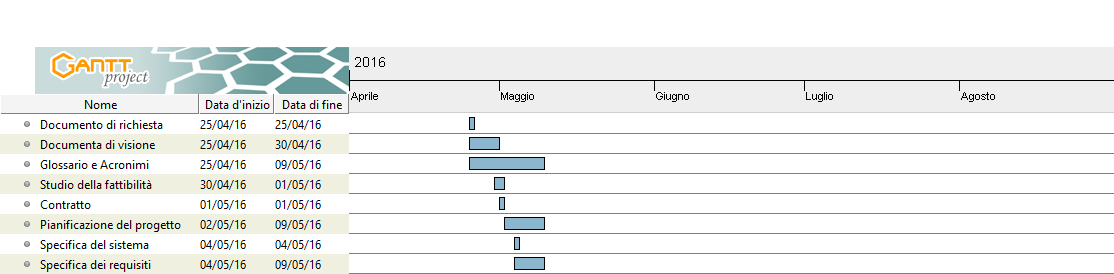
\includegraphics[width=\linewidth]{diagrammaGantt/DiagrammaGantt}
\end{center}
\end{landscape}

\newdate{pianuno}{3}{05}{2016}
\newdate{piandue}{4}{05}{2016}
\newdate{piantre}{15}{05}{2016}
\section{Revisioni}
\begin{center}
    \begin{tabular}{lll}
        \toprule
        	\tabhead{Versione} & \tabhead{Data} & \tabhead{Descrizione} \\
		\cmidrule(l{\cmidrulekern}r{\cmidrulekern}){1-3}
	        1.0 & \displaydate{pianuno} & Prima versione \\
	        1.1 & \displaydate{piandue} & Aggiunta iterazione 02 \\
	        1.2 & \displaydate{piantre} & Riorganizzate pianificazione \\
        \bottomrule
    \end{tabular}
\end{center}
